% $Id$

\chapter{Introduction}
\label{chap:intro}
\minitoc

%==========================
\section{Background}
%==========================

Advances in neuroimaging techniques have radically changed the way neuroscientists address questions about functional anatomy, especially in relation to behavioural and clinical disorders. Many questions about brain function, previously investigated using intracranial electrophysiological recordings in animals can now be addressed non-invasively in humans. Such studies have yielded important results in cognitive neuroscience and neuropsychology. Amongst the various neuroimaging modalities available, Magnetic Resonance Imaging (MRI) has become widely used due to its relatively high spatial and temporal resolution, and because it is safe and non-invasive. By selecting specific MRI sequence parameters, different MR signals can be obtained from different tissue types, giving images with high contrast among organs, between normal and abnormal tissues and/or between activated and deactivated brain areas. MRI is often sub-categorized into structural MRI (MRI) and functional MRI (fMRI). Examples of other of imaging modalities that measure  brain signals are Positron Emission Tomography (PET), ElectroEncephaloGraphy (EEG) recordings and MagnetoEncephaloGraphy (MEG) recordings. Neuroimaging data are inherently multivariate, since each measure (scan or recording) contains information from thousands of locations (e.g. voxels in MRI or electrodes in EEG). Considering that most brain functions are distributed processes involving a network of brain regions, it would seem desirable to use the spatially distributed information contained in the data to give a better understanding of brain functions in normal and abnormal conditions. 

The typical analysis pipeline in neuroimaging is strongly rooted in a mass-univariate statistical approach, which assumes that activity in one brain region occurs independently from activity in other regions. Although this has yielded great insights over the years, specially in terms of function localization, and continues to be the tool of choice for data analysis, there is a growing recognition that the spatial dependencies among signal from different brain regions should be properly modelled. The effect of interest can be subtle and spatially distributed over the brain - a case of high-dimensional, multivariate data modelling for which conventional tools may lack sensitivity. 

Therefore, there has been an increasing interest in investigating this spatially distributed information using multivariate pattern recognition approaches, often referred to as  multi-voxel pattern analysis (MVPA) (see  \cite{Norman2006},  \cite{Haynes2006} and \cite{Pereira2009}). Where pattern recognition has been used in neuroimaging, it has led to fundamental advances in the understanding of how the brain represents information and has been applied to many diagnostic applications. For the latter, this approach can be used to predict the status of the patient scanned (healthy vs. diseased or disease A vs. B) and can provide the discriminating pattern leading to this classification. Pattern recognition techniques can also be used to identify relationships between patterns of brain structure or activity and continuous measures such as age or a clinical score. Such information can then be used to predict individual-level measures for new individuals (i.e. regression models).

Several active areas of research in machine learning are crucially important for the difficult problem of neuroimaging data analysis: modelling of high-dimensional multivariate time series, sparsity, regularisation, dimensionality reduction, causal modelling, and ensembling to name a few. However, the application of pattern recognition approaches to the analysis of neuroimaging data is limited mainly by the lack of user-friendly and comprehensive tools available to the fundamental, cognitive, and clinical neuroscience communities. Furthermore, it is not uncommon for these methods to be used incorrectly, with the most typical case being improper separation of training and testing datasets.


%==========================
\section{Methods}
%==========================

PRoNTo (Pattern Recognition for Neuroimaging Toolbox) is a toolbox based on pattern recognition techniques for the analysis of neuroimaging data. Statistical pattern recognition is a field within the area of machine learning which is concerned with automatic discovery of regularities in data through the use of computer algorithms, and with the use of these regularities to take actions such as classifying the data into different categories \cite{Bishop2006}. In PRoNTo, brain images are treated as spatial patterns and statistical learning models are used to identify statistical properties of the data that can be used to discriminate between experimental conditions or groups of subjects (classification models) or to predict a continuous measure (regression models).


PRoNTo is \matlab based and includes five main modules: `Data \& Design', `Prepare feature set', `Specify model', `Run model' and `Compute weights'. The results can displayed in terms of the performance of the estimated model, as well as in terms of model parameters. Additional review options enable the user to review information about the data, features and models. All modules were implemented using a graphical user interface (GUI) and the MATLAB Batch System. Using the MATLAB Batch System the user can run each module as batch jobs, which enables a very efficient analysis framework.  All information about the data, experimental design, models and results are saved in a structure called PRT. PRoNTo also creates additional files during the analysis that are described in details in the next chapters.

The toolbox code will be distributed for free, but as copyright software under the terms of the GNU General Public License as published by the Free Software Foundation. 

\subsection{Inputs and preprocessing}

In terms of neuroimaging modalities, PRoNTo accepts NIFTI files. Mostly designed to analyse structural and functional Magnetic Resonance Imaging and PET, it can be used on any dataset converted to a NIFTI file. It assumes that the neuroimaging data has been previously pre-processed using SPM (\url{http://www.fil.ion.ucl.ac.uk/spm/}) or a similar software for neuroimaging analysis. In general, raw fMRI data should be previously corrected for movement artefact (realigned) and time difference in slice acquisition (slice time correction), mapped to a common template (normalized) and spatially smoothed. The normalisation and spatial smoothing steps might not be necessary for single subject analysis.  

In addition the General Linear Model (GLM) can be applied as a pre-processing step for pattern recognition analysis. In this case, the GLM coefficients (e.g. beta images in SPM) will correspond to the spatial patterns. Using beta images should be preferred in the case of event-related designs with short inter-stimulus time and/or event duration to better take into account the Haemodynamic Response Function (HRF). \textbf{Important note}: Beta images output by SPM contain NaNs (Not a Number) values in some voxels. For better performance of the model, a mask should be created to exclude the corresponding voxels from the analysis. Practically, a mask should be built (e.g. using SPM imcalc batch or a script provided in `utils') to specify which voxels have scalar values (1 in mask) or NaN or 0 value (0 in mask). The updated mask should then be input in the Data \& Design window. To ease this extra preprocessing step, a script is provided in \textit{your PRoNTo folder/utils}. It takes as inputs the images (i.e. beta images in nifti format), the mask to update (e.g. SPMnoeyes.nii provided in \textit{your PRoNTo folder/mask}) and the directory to save the updated mask. Inputs are optional, and just typing in the \matlab command: prt\_utils\_update\_mask will ask for the different inputs using file and path selectors.

Raw structural MRI data should be previously mapped to a common template (normalized) and spatially smoothed. Raw PET data should be realigned, normalized and smoothed. PET data is also usually scaled. This operation can be performed before hand or during the building of the feature set.

%In the current version of the software, regression models and regressing out effect of covariates from the data is provided only when selecting images by scans (i.e. for one image per subject). Therefore, we suggest that users interested in removing covariates from datasets with a (fMRI) design perform a GLM analysis before hand and input the derived beta images as patterns.

\subsection{Machine learning algorithms}

In PRoNTo different pattern recognition algorithms correspond to different machines. The machine library in PRoNTo v2 includes four classification models: Support Vector Machine (\cite{Cristianini2000}, \cite{Mourao-Miranda2007}), Gaussian Process Classifier (binary and multiclass, \cite{Rasmussen2006}, \cite{Marquand2010}) and L1-Multiple Kernel Learning \cite{Rakotomamonjy2008}. Four regression models are available: Kernel Ridge Regression \cite{ShaweTaylor2004}, Relevance Vector Regression \cite{Tipping2001}, Gaussian Process Regression \cite{Rasmussen2006} and L1-Multiple Kernel regression \cite{Rakotomamonjy2008}. New machines will be added to the library in future versions of the toolbox. %, Random Forest \cite{Geurts2006}

PRoNTo should facilitate the interaction between machine learning and neuroimaging communities. On one hand the machine learning community should be able to contribute to the toolbox with novel published machine learning models. On the other hand the toolbox should provide a variety of tools for the neuroscience and clinical neuroscience communities, enabling them to ask new questions that cannot be easily investigated using existing statistical analysis tools. 


%=====================
\section{Installing \& launching the toolbox}
%=====================
\label{sec:Installation}

In order to work properly, PRoNTo requires 2 other softwares:
\bi
\item a recent version of \matlab. We used versions 7.5 (R2007b) to 8.3 (R2014a) to develop PRoNTo, and it will not work with earlier versions\footnote{Any later \matlab~version should work, {\it in theory}.}. 
\item SPM8\cite{SPM8} installed on your computer\footnote{SPM8 can be dowloaded from the following website: \url{http://www.fil.ion.ucl.ac.uk/spm/software/}. You should install it in a suitable directory, for example {\tt C:\bslash SPM8\bslash }, then make sure that this directory is on the \matlab path. No need to include the subdirectories!}. SPM12b and SPM12 are also supported.
\ei

PRoNTo latest public version can be downloaded, after registration, from the following address: \url{http://www.mlnl.cs.ucl.ac.uk/pronto/prtsoftware.html}.

\textbf{Important note}: if you already have a version of SPM on your computer, please download the latest updates from the website. Various bugs, especially in terms of weight visualization, arise from out of date SPM versions.

\subsection{Installation}
%--------------------------------------

After downloading the zipped file containing PRoNTo, the installation proceeds as follow:
\begin{enumerate}\addtolength{\itemsep}{-1\baselineskip}
\item	Uncompress the zipped file in your favourite directory, for example {\tt C:\bslash PRoNTo\bslash };\\
\item	Launch \matlab ;\\
\item	Go to the ``{\tt File}'' menu $\rightarrow$ ``{\tt Set path}'';\\
\item	Click on the ``{\tt Add folder}'' button and select the PRoNTo folder, i.e. {\tt C:\bslash PRoNTo\bslash } if you followed the example;\\
\item	Click on save.
\end{enumerate}

Some routines, in particular the 'machines', are written in C++ ({\tt .cpp} files) for increased efficiency. We are trying to provide these compiled routines for the usual Operating Systems (OS's) such as: Windows XP (32 bits), Windows 7 (64 bits), Mac OS 10, Linux (32 and 64 bits). If your OS is not listed or routines do not work properly then you should compile the routines for your specific OS\footnote{you can also contact us and we'll try to come up with a solution for your system.}. 

\subsection{Launching and batching}
%--------------------------------------

Once installed, there are three ways to call up PRoNTo functionalities.
To launch the toolbox GUI, just type {\tt prt} or {\tt pronto} at the \matlab \ prompt and the main GUI figure will pop up, see Fig.~\ref{fig:mainGUI}. From there on simply click on the processing step needed (see Part \ref{sec:GUI} of this manual). Most functions of PRoNTo have been integrated into the {\tt matlabbatch} batching system \cite{matlabbatch} (like SPM8) and the batching GUI is launched from the main GUI by clicking on the {\tt Batch} button  (see Part \ref{sec:BATCH} of this manual).
Of course most tools can also be called individually by calling them directly from the \matlab \ prompt, or for scripting in a {\tt .m} file  (see Part \ref{sec:ADVTOP} of this manual).

\begin{figure}[!htbp]
  \begin{center}
      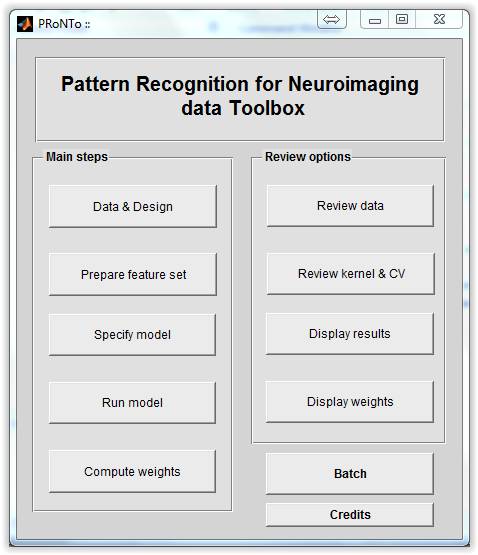
\includegraphics[height=7cm]{images/fig2_main_prt.png}
   \caption{Main GUI interface: each button launches a specific processing step.}
    \label{fig:mainGUI}
  \end{center}
\end{figure}	

\subsection{Troubleshooting}
%--------------------------------------
\subsubsection{Compiling libsvm}
Some problems when using SVMs might arise due to  libsvm, in which case, you might need to compile it on your own. The first thing that needs to be done is to download the desired libsvm version (usually the latest one) from the following website: \url{http://www.csie.ntu.edu.tw/~cjlin/libsvm/}. Then, the process will depend on your operating system.

If the steps described bellow do not work, please refer to the {\tt README} file that comes with libsvm.

\paragraph{Microsoft Windows}
\begin{itemize}
    \item Make sure you have a C++ compiler install. If not, you can install Microsoft Visual C/C++;
    \item Copy the libsvm folder to the `machines' directory of your PRoNTo instalation\\(e.g. C:\bslash PRoNTo\bslash machines\bslash);
    \item Open a DOS command window and change to the libsvm folder in the previous step ({\tt cd C:\bslash PRoNTo\bslash machines\bslash libsvm-3.17\bslash}). If the environment variables of VC++ have not been set, run the following command:\\{\tt C:\bslash Program Files\bslash Microsoft Visual Studio 10.0\bslash VC\bslash bin\bslash vcvars32.bat}. This command might be different, depending on the path of your Visual Studio installation;
    \item In the libsvm folder run the command: {\tt nmake -f Makefile.win clean all} 
    \item If no errors appear, open MATLAB;
    \item Change to the `matlab' folder inside the libsvm folder (e.g. C:\bslash PRoNTo\bslash machines\bslash libsvm-3.17 \bslash matlab\bslash);
    \item Run {\tt make} in the MATLAB Command Window. If there are no errors, you have just successfully compiled libsvm to be used with MATLAB.
\end{itemize}

Remember, if you want to use the version that you have just compiled, you have to add the libsvm folder to your path in MATLAB. If you have more than one libsvm folder inside the `machines' folder, please remove one of them from the MATLAB path. You should only have one libsvm folder in your path.


\paragraph{Unix (Mac OS or Linux)}

\begin{itemize}
    \item Make sure you have a C++ compiler installed. If you are using Mac OS, please install `Xcode'. On Linux systems, you should already have `gcc' installed;
    \item Copy the libsvm folder to the `machines' directory of your PRoNTo instalation\\(e.g. {\tt /home/<username>/PRoNTo/machines/});
    \item Open a terminal window and change to the `machines' directory: {\tt cd PRoNTo/machines/}
    \item Compile libsvm by running the following command: {\tt make}
    \item If no errors appear, open MATLAB;
    \item Change to the `matlab' folder inside the libsvm folder (e.g. PRoNTo/machines/libsvm-3.17/matlab/);
    \item Run {\tt make} in the MATLAB Command Window. If there are no errors, you have just successfully compiled libsvm to be used with MATLAB.
\end{itemize}

Remember, if you want to use the version that you have just compiled, you have to add the libsvm folder to your path in MATLAB. If you have more than one libsvm folder inside the `machines' folder, please remove one of them from the MATLAB path. You should only have one libsvm folder in your path.

%==========================
\section{What's new?}
%==========================
\subsection{Version 2.1}
This version of the toolbox is released mainly to provide bug fixes for version v2.0. One feature is also added: removing confounds in kernel space for predictions and in the original space for weight computation. A detailed description can be find: \url{http://www.cs.ucl.ac.uk/fileadmin/UCL-CS/research/Research_Notes/RN_17_09_ARJMM.pdf}. 
\subsection{Version 2.0}
This version of the toolbox (2015) aims at providing multiple new functionalities, including:
\begin{itemize}
\item \textbf{Build one kernel per modality}: When there are multiple modalities in the same dataset, it is now possible to build one kernel per modality and use them in the same model later on. If this option is not chosen, the selected modalities can still be concatenated as additional samples/examples or sessions (if they have the same dimensions) or used separately.
\item \textbf{Build one kernel per region}: It is also possible to specify an atlas, comprising regions of interest (ROIs) as defined by values in the atlas ranging from 1 to \textit{number of ROIs}. For each anatomically defined ROI, a kernel will be built taking into account the multivariate pattern within the region. It is possible to use this feature in combination with the previous one (e.g. one kernel per region and per modality, or concatenate modalities as additional samples and build one kernel per region).
\item \textbf{New machines}: The list of available machines was extended, and now includes L1-Multiple Kernel Learning (MKL, classification and regression). The latter corresponds to a hierarchical model defined by weights at two levels: the voxel level and the kernel level (i.e. ROI and/or modality).
\item \textbf{Flexible cross-validation}: A GUI is provided to manually specify a custom cross-validation matrix. It allows to either specify a basis (e.g. leave-one-subject-out), load a .mat or specify the number of folds. Then the user can, for each fold, select which examples are part of the training set, test set, or won't be used. The resulting matrix can be saved for further use.
\item \textbf{Nested cross-validation for hyperparameter optimization}: It is now possible to optimize the hyperparameter(s) of some machines (e.g. the soft-margin parameter, C, in SVM) using a nested cross-validation (CV) framework. The number of folds in the nested cross-validation, used only to estimate the value of the hyperparameter leading to the highest performance, does not need to be the same as the `outer' cross-validation (i.e. the one estimating the final model performance). For example, to decrease computational expenses, the nested CV can be a 4-fold CV while the outer CV can be a leave-one-out.
\item \textbf{Display results}: The display of the results was divided into two modules (Display Results and Display Weights). This allows to review the model performance in one window, with all the statistics. A new graph displaying the effect of the hyperparameter (if optimized) was also included.
\item \textbf{Weights per ROI}: For each model it is possible to build images representing the weights per voxel and also images summarising the weights per regions of interest as defined by an atlas. If an MKL model was built on ROIs, the contribution of each ROI (regional weight) is explicitly derived. On the other hand, if a simple kernel model was selected (e.g. SVM on the whole brain), the weights per voxel will be averaged (in absolute value) within each region, as defined by an atlas specified by the user. In both cases, an additional image, with weights per ROI, is created and saved.
\item \textbf{Display weights}: The weights of each model can be displayed at the voxel level in this window. If weights per ROI were derived (either summarized or from an MKL on ROIs), weights per region can be displayed as an image, as well as in a sorted list of regions. The same applies for MKL models on multiple modalities. A histogram is also displayed representing the contribution/weight of each ROI/modality to the model. The table can be exported as text for future use in publications/communications.
\end{itemize}

\subsection{Version 1.1}
In 2012, PRoNTo v1.1 was released mainly to provide bug fixes for version v1.0. Two features were also added:
\begin{itemize}
\item automatic compiling of the machines (in particular: no more issues with SVM, nor with Matlab toolboxes and paths).
\item k-folds Cross-Validation (CV): specify the number of folds or set it to 1 for half-half CV (train on first half, test on second).
\end{itemize}

\subsection{Version 1.0}
Launched in 2011, this version of PRoNTo allows to perform all the analysis steps, from Data \& Design to computing the weights for three classification machines (SVM, binary and multi-class GP) and two regression machines (KRR, SVR).

\subsection{How to cite}
%--------------------------------------
Please cite \cite{Schrouff2013} when using PRoNTo analyses in any type of publication. In addition, Multiple Kernel Learning analyses should refer to a second paper (submitted, tba)\footnote{When the paper gets accepted, this section will be updated and the paper will be listed in the documentation section of the website}. Meanwhile, please cite \cite{Schrouff2014} for MKL analyses and \cite{Schrouff2013a} for a posteriori weight summarization using atlas-defined regions of interest. 

%==========================
\section{Main contributors}
%==========================
PRoNTo is  developed by the Machine Learning \& Neuroimaging Laboratory, Computer Science department, University College London, UK (\url{ http://www.mlnl.cs.ucl.ac.uk}) and associated researchers.

The main contributors, in alphabetical order, are: 
\begin{description}
	\item[Dr. John Ashburner] is a Professor of Imaging Science at the Wellcome Trust Centre for Neuroimaging at the University College London Institute of Neurology. He is mainly interested in modelling brain anatomy from MR scans, and more recently in applying pattern recognition methods to make predictions about individual subjects. He is a co-developer of the SPM software (intra- and inter-subject registration, tissue classification, visualization and image file formats), which is used internationally by thousands of neuroimaging researchers. He has a Web of Science h-index of 63.  He did not contribute any actual code to PRoNTo, but he did attend many of the meetings;
    \item[Dr. Carlton Chu] is a research scientist at  Google DeepMind. Before joining DeepMind, he was a research fellow in brain imaging at the National Institute of Mental Health (NIMH), NIH. He received the B.Eng. degree (1\textsuperscript{st} class Honours) from Auckland University, in 2002 and the master of Biomedical Engineering from University of New South Wales, in 2004. Carlton obtained a PhD in Neuroimaging method from University College London in 2009, working in the statistical methods group at the Wellcome Trust Centre for Neuroimaging, creators of the famous ``SPM'' program. There he developed innovative pattern recognition methods to automatically detect the early stages of neurodegenerative diseases such as Alzheimer's and Huntingdon's from structural brain images. In 2007, Carlton won the first prize in the 2nd Pittsburgh Brain Activity Interpretation Competition (PBAIC), a prestigious international competition involving the application of machine learning to the problem of classification of brain activity. He led a small research team to victory, acclaim from peers in the field, and the \$10K first prize. His current research interests include image segmentation using convolutional neural networks and applications of deep-learning. Carlton was involved in the development of PRoNTo version 1.0;
	\item[Dr. Andre Marquand] is an Junior Principal Investigator at the Donders Institute for Brain Cognition and Behaviour and a Lecturer at the Institute of Psychiatry, Psychology and Neuroscience, King's College London.  His research focuses on the application of probabilistic machine learning techniques to neuroimaging data, particularly for clinical applications. His recent work includes the development of multi-class, multi-task and multi-modality pattern classification methods that offer many advantages over current techniques including more sensitive and specific detection of disease effects;
	\item[Dr. Janaina Mourao-Miranda] is a Wellcome Trust Senior Research Fellow at the Centre for Computational Statistics and Machine Learning (CSML), UCL.  Over the past years her research has involved developing and applying pattern recognition methods to analyze neuroimaging data, in particular brain activation and structural patterns that distinguish between controls and patients. Her current research focuses on developing machine-learning models to investigate complex relationships between neuroimaging data and multidimensional descriptions of mental health disorders. She has been coordinating the PRoNTo developments and contributed to PRoNTo versions 1.0, 1.1 and 2.0;
	\item[Mr. Joao M. Monteiro] is a former MPhil/PhD Student at University College London under the supervision of Prof. John Shawe-Taylor and Dr. Janaina Mourao-Miranda. His research focuses on the application of unsupervised machine learning methods to neuroimaging. He contributed to PRoNTo versions 1.1 and 2.0;
	\item[Dr. Christophe Phillips] is FRS-FNRS Research Associate at the Cyclotron Research Centre and adjunct Assistant Professor at the Department of Electrical Engineering and Computer Science, University of Li\`ege, Belgium. His research focuses on the processing of multi-modal neuroimaging data. Recent work within the field of ``brain decoding'' aimed at distinguishing between levels of consciousness in unresponsive patients or between typical and atypical Parkinson Disease patients using Positron Emission Tomography (PET) imaging, as well as tracking mnesic traces in trained healthy subjects with fMRI;
	\item[Dr. Jonas Richiardi] is a Marie Curie researcher at the University of Geneva (Department of Fundamental Neuroscience). His research interests include the combination of imaging modalities with other biological information sources including genomic data, learning with graphs, machine learning for neuroimaging, brain connectivity / resting-state data analysis, interpretability of brain decoding results, and functional biomarkers. He has been involved with the organization of the workshop on Pattern Recognition in NeuroImaging since the beginning;
	\item[Dr. Jane Rondina] is a research fellow at the University College London Institute of Neurology. Previously, she was a post-doctoral research associate at the Centre for Neuroimaging Sciences, King's College London. In the past years, her research has involved application of pattern recognition methods to neuroimaging data and development of a stability-based method for feature selection and mapping in neuroimaging. Her current research focuses on prognosis and prediction of treatment response, mainly addressing approaches to combine complementary information from different imaging modalities and other sources of data (clinical, demographic and genetic). She contributed to the development of PRoNTo version 1.0. She is also involved in incorporation of new resources for version 3.0;
	\item[Dr. Maria J. Rosa] is an imaging scientist at IXICO, plc. Before, she was a Post-Doctoral Research Fellow at the Institute of Psychiatry, King's College London (KCL) and a Wellcome Trust post doctoral research associate at the Centre for Computational Statistics and Machine Learning (CSML), UCL. Maria's main area of work is the development and application of machine learning and multivariate methods to neuroimaging data. She did her PhD at the Wellcome Trust Centre for Neuroimaging, UCL. She contributed to PRoNTo versions 1.0, 1.1 and 2.0;
	\item[Dr. Jessica Schrouff] got her PhD from the University of Li\`ege, under the supervision of Dr. C. Phillips. She is a post-doctoral researcher at the Laboratory of Behavioral and Cognitive Neuroscience, Stanford University. Her research focuses on the detection and characterization of memory traces in resting state wakefulness using machine learning techniques, based on fMRI data (Ph.D. thesis) and intracranial EEG recordings. She contributed to PRoNTo versions 1.0, 1.1 and 2.0. She has also started adapting the toolbox for analysis of electrophysiological recordings (version 3.0);
	\item[Dr. Tong Wu] got her PhD from the University of Queensland in Australia, under supervision of Dr. Tianzi Jiang, Dr. David Reutens and Dr. Simone Bosshard. She is a post-doctoral researcher in Centre for Medical Image Computing (CMIC) at the University College London. Her research focus during PhD was resting-state mouse fMRI in both wild type mice and a schzophrenia mouse model. She contributed to PRoNTo version 2.1.    
\end{description}

We also thank students and post-docs for their help in testing the software and writing this manual: Dr. Liana Lima Portugal, Liane Canas, Dr. Ana Regia Neves, Rochelle Silva, Dr. Orlando Fernandes Junior and Dr. Qinquan Gao. 

%==========================
\section{Acknoweldgements}
%==========================
PRoNTo is the deliverable of a Pascal Harvest project coordinated by Dr. J. Mourao-Miranda and its development was possible with the financial and logistic support of 
\begin{itemize}
\item the Department of Computer Science, University College London  (\url{http://www.cs.ucl.ac.uk});
\item the Wellcome Trust (\url{http://www.wellcome.ac.uk/}) under grants no. WT086565/Z/08/Z and no. WT102845/Z/13/Z;
\item PASCAL2 (\url{http://www.pascal-network.org}) and its HARVEST programme;
\item the Fonds de la Recherche Scientifique-FNRS (\url{http://www.fnrs.be}), Belgium;
\item Funda\c{c}\~{a}o para a Ci\^{e}ncia e Tecnologia - FCT (\url{http://www.fct.pt}), Portugal;
\item Swiss National Science Foundation (PP00P2-123438) and Center for   Biomedical Imaging (CIBM) of the EPFL and Universities and Hospitals  of Lausanne and Geneva.
\item The EU Marie Curie Action under grant FP7-PEOPLE-2011-IOF \# 299500.
\item The Laboratory of Behavioral and Cognitive Neuroscience, Stanford University.
\end{itemize}

%PRoNTo is written for MATLAB X.Y (R20ZZb) and onwards. Some routine may need to be compiled for your specific OS.
